% \begin{document}
\chapter{Probabilistic approach}
\section{core idea}
we have two main points of views:
\begin{itemize}
    \item \textbf{traditional view}: we wanna to approximate a function $f:X\to X$
    \item \textbf{Probabilist view}: we wanna compute probablilities: $p: P( Y\mid  X)$
\end{itemize}
\subsection{Probs basics}
\subsubsection{Random variables}
A random variables $X$ represents an oyt come about which we're ncertain
\ex{Random variables}{
\begin{itemize}
    \item $X=$\texttt{true} if a randomly drawn stdent is male
    \item $X=$ first name of the student
    \item $X=$\texttt{true} if a randomly drawn stdent have the same birthday
\end{itemize}
}
 
Formal def:
\dfn{Probs variables}{
    the set $\Omega$ of the possible outcomes is called the sample space. It is said random variable a measurable function over $\Omega$:
    \begin{itemize}
        \item Discrete: $\Omega \to \{m,f\}$
        \item Continuos: $\Omega\to \mathbb{R}$
    \end{itemize}
}
 
\dfn{Probs def}{
    it is defined $P(X)$ is the fraction of times $X$ is true in repeated runs of the same experiment.
}

\nt{
    The definition requires that all samples 
}

Pay attention:
\wc{
    bad examples
}{
    Sample space, let $\Omega$ be a space made the possibile sum:
    \[
        \Omega = \{2,3,4,\dots, 12\}
    \]
    Problem: not all sums are equally likely! It should be:
    \[
        \begin{array}{c}
            P(sum = 2) = 1/11\\
            P(sum = 7) = 1/11
        \end{array}
    \]
    but in reality:
    \begin{itemize}
        \item Sum = 2: can only happen one way: $(1,1)$
        \item Sum = 7: can happen six ways:$(1,6), (2,5), (3,4), (4,3), (5,2), (6,1)$
    \end{itemize}

    so 
    \[
        P(sum = 2) \neq P(sum = 7)
    \]
}

A correct approach is 
\clm{correct approach}{}{
    Be $\Omega = {(1,1), (1,2), (1,3), ..., (6,5), (6,6)}$, where $|\Omega|=36 $outcomes

    each pair has equally probability = $\frac{1}{36}$
    
    Now here is a correctly computing:
    \[
        \begin{array}{c}
            P(sum = 2) = \frac{|{(1,1)}|}{36} = \frac{1}{36}\\
            P(sum = 7) = \frac{|{(1,6), (2,5), (3,4), (4,3), (5,2), (6,1)}|}{36} = \frac{6}{36}
        \end{array}
    \]
}

\subsubsection{The Axioms of Probability Theory}
These are the fundamental rules that make probability a "reasonable theory of uncertainty":

\ax{Axioms of probability theory}{
    \begin{align}
        &\text{(1) Non-negativity: } && 0 \leq P(A) \leq 1 \quad \text{for all events } A. \\
        &\text{(2) Normalization: } && P(\Omega) = 1. \\
        &\text{(3) Countable additivity: } && 
        \text{If } A_1, A_2, \dots \text{ are disjoint, then } 
        P\!\left(\bigcup_{i=1}^\infty A_i\right) = \sum_{i=1}^\infty P(A_i).
    \end{align}
}

Then:

\cor{consequences of the axioms}{
\begin{itemize}
    \item Monotonicity: If $A \subseteq B$, then $P(A) \le P(B)$
    \item Union rule (for two events): $P(A \cup B) = P(A) + P(B) - P(A \cap B)$
    \item $P(True) = 1$
    \item $P(False) = 0$
\end{itemize}
}

\begin{center}
    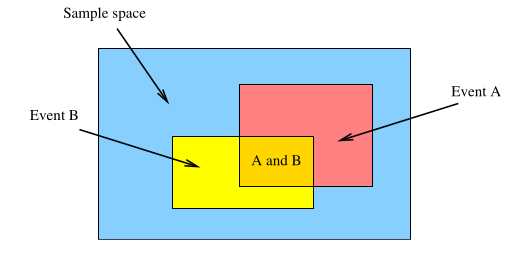
\includegraphics[width=5cm]{probs_ax.png}
\end{center}

\subsubsection{Derivied theorems}
\cor{Complement Rule
}{
    \[
        P(\lnot A) = 1- P(A)
    \]
}
\pf{Dm}{
\[
P(A \cup \neg A) = P(A) + P(\neg A) - P(A \cap \neg A)
\]

But: 
\[
P(A \cup \neg A) = P(\text{True}) = 1
\quad \text{and} \quad
P(A \cap \neg A) = P(\text{False}) = 0
\]

Therefore:
\[
1 = P(A) + P(\neg A) - 0
\quad \implies \quad
P(\neg A) = 1 - P(A) \qed
\]

}

\cor{Partition Rule}{
    \[
        P(A) = P(A \cap B) + P(A \cap \neg B)
    \]
}
\pf{Proof}{
    \[
\begin{aligned}
A &= A \cap (B \cup \neg B) &\text{[since $B \cup \neg B$ is always True]}\\
  &= (A \cap B) \cup (A \cap \neg B) &\text{[distributive law]}
\end{aligned}
\]

Hence,
\[
\begin{aligned}
P(A) &= P((A \cap B) \cup (A \cap \neg B)) \\
     &= P(A \cap B) + P(A \cap \neg B) - P((A \cap B) \cap (A \cap \neg B)) \\
     &= P(A \cap B) + P(A \cap \neg B) - P(\text{False}) \\
     &= P(A \cap B) + P(A \cap \neg B)
\end{aligned}
\]

}
\subsubsection{Multivalued Discrete Random Variables}
\dfn{
    k-value Discrete Random Variables
}{
    A random variable $A$ is \textit{$k$-valued discrete} if it takes exactly one value from 
    \[
    \{\nu_1, \nu_2, \dots, \nu_k\}.
    \]
}

\mprop{Key proprieties}{
    \begin{enumerate}
    \item \textbf{Mutual exclusivity:} For $i \neq j$,
    \[
        P(A = \nu_i \cap A = \nu_j) = 0
    \]

    \item \textbf{Exhaustiveness:}
    \[
        P(A = \nu_1 \cup A = \nu_2 \cup \dots \cup A = \nu_k) = 1
    \]
\end{enumerate}

}

\subsubsection{Conditional Probability}
\dfn{Conditional probs}{
    The Conditional probs of the event $A$ \textit{given} the event $B$ is defined as the quantity
    \begin{center}
        \begin{math}
            P(A\mid B) = \frac{P(A\cap B)}{P(B)}            
        \end{math}
    \end{center}
}

\cor{Cahin roule}{
    \[
        P(A\cap B) = P(B)P(A\mid  B)= P(A) P(B\mid A)
    \]
}
\subsubsection{Independent Events}
\dfn{Independent Events}{
    Events $A$ and $B$ are independent when:
    \begin{center}
        \begin{math}
            P(A\mid  B) = P(B)
        \end{math}
    \end{center}
}
(Meaning: B provides no information about A.)
\cor{consequences}{
    \begin{itemize}
        \item $P(A\cap b) = P(A)P(B)$ (from chail roule)
        \item $P(B|A) = P(B)$ (symmetry)
    \end{itemize}
}

\subsubsection{Bayes' Rule: The Heart of Probabilistic ML (ok chat... really?)}
\thm{Bayes's roule}{
    Now we have Bayes roule
    \begin{center}
        \begin{math}
            P(A\mid  B) = \frac{P(A)  P(B\mid A)}{P(B)}
        \end{math}
    \end{center}
}
\pf{Proof}{
    It's true by the chain roule that: $P(A \cap B) = P(B)  P(A\mid B)$. It's true also the reverse case $P(A \cap B) = P(B) · P(A\mid B)$.

    Since both expressions equal $P(A \mid B)$, they must equal each other:
    \[
        P(A)  P(B\mid A) = P(B)  P(A\mid B) 
    \]
    that it's equal to
    \[
        P(A\mid B) =\frac{[P(A)  P(B\mid A)]}{P(B)}
    \]
}
\ex{The trousers problem}{
    Setup:
    \begin{itemize}
        \item 60\% of students are boys, 40\% are girls
        \item girls wear in the same number skirt and trousers
        \item boys only wear trousers
    \end{itemize}
    If we see a student wearing trousers, what is the probability that is a girl?
}
\pf{Solution}{
    The probs a priori that a strudent is a girl is
    \[
        P(G) = \frac{2}{5}
    \]
    the probability that a student wears trousers is
    \[
        P(T) = \frac{1}{5} + \frac{3}{5} = \frac{4}{5}
    \]
    the probability that a student wear trousers, given that the student is a girl, is
    \[
        P(T\mid G) = 1/2
    \]
    So 
    \[
        P(G\mid T) =\frac{p(G)p(T\mid G)}{P(T)}=\frac{2/5\cdot 1/2}{4/5} = 1/4
    \]
}

\paragraph{Machine Learning Form}
\paragraph{Machine Learning Form}
For discrete $Y$ with values $\{y_1, y_2, \ldots, y_m\}$ and $X$ with values $\{x_1, x_2, \ldots, x_n\}$:
\[
P(Y = y_i \mid X = x_j) = \frac{P(Y = y_i) \cdot P(X = x_j \mid Y = y_i)}{P(X = x_j)}
\]

\textbf{Expanding the denominator:}
\begin{align*}
P(X = x_j) &= \sum_{i} P(X = x_j, Y = y_i) \quad \text{[sum over all $Y$ values]} \\
           &= \sum_{i} P(Y = y_i) \cdot P(X = x_j \mid Y = y_i) \quad \text{[chain rule]}
\end{align*}

\textbf{Complete Bayes' Rule:}
\[
P(Y = y_i \mid X = x_j) = \frac{P(Y = y_i) \cdot P(X = x_j \mid Y = y_i)}{\sum_{i} P(Y = y_i) \cdot P(X = x_j \mid Y = y_i)}
\]

\textbf{Terminology:}
\[
\underbrace{P(Y \mid X)}_{\text{posterior}} = \frac{\overbrace{P(X \mid Y)}^{\text{likelihood}} \cdot \overbrace{P(Y)}^{\text{prior}}}{\underbrace{P(X)}_{\text{marginal}}}
\]

\begin{itemize}
    \item \textbf{Posterior} $P(Y \mid X)$: What we want -- probability of $Y$ given observed $X$
    \item \textbf{Likelihood} $P(X \mid Y)$: How likely is $X$ if $Y$ is true?
    \item \textbf{Prior} $P(Y)$: What we believed before seeing $X$
    \item \textbf{Marginal} $P(X)$: Overall probability of observing $X$ (normalization constant)
\end{itemize}

\textbf{Alternative form:}
\[
\text{Posterior} = \frac{\text{Likelihood} \cdot \text{Prior}}{\text{Marginal Likelihood}}
\]
where:
\[
\text{Marginal} = \sum_{Y} P(X \mid Y) \cdot P(Y)
\]

The term ``marginal'' means we've \textbf{marginalized} (integrated/summed) over $Y$.

\section{The Joint Distribution}

\dfn{Joint Distribution}{
    Let $X_1, X_2,\dots, X_n$ be discrete random variables. The \textit{joint probability distribution} (or \textit{joint distribution}) of these variables is the function:
    \begin{center}
        \begin{math}
            P(X_1 = x_1, X_2 = x_2, \dots, X_n = x_n)
        \end{math}
    \end{center}

    which assigns to every possible combination of values \( (x_1, x_2, \dots, x_n) \) the probability that the random variables simultaneously take those values.

    Formally, for discrete variables, the joint distribution satisfies:
    \begin{itemize}
        \item \( 0 \leq P(x_1, x_2, \dots, x_n) \leq 1 \) for all \( (x_1, \dots, x_n) \)
        \item \( \sum_{x_1} \sum_{x_2} \cdots \sum_{x_n} P(x_1, x_2, \dots, x_n) = 1 \)
    \end{itemize}
}

Let's see an example
\ex{Joint distribution}{
    \begin{itemize}
        \item build a table with all possible combinations of values of random variables (features)
        \item compute the probability for any different combination of values
    \end{itemize}

    \begin{center}
        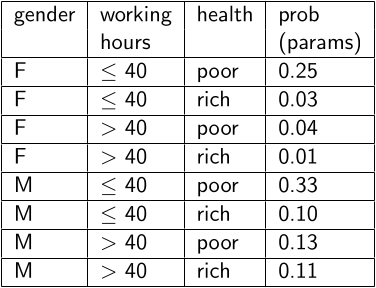
\includegraphics[width=6pt]{jd_img.png} % the table of the document
    \end{center}

    This table is the "Joint distribution"!

    Having that we may compute the probability of any event expressible as a logical combination of the features, with this formula
    \[
        P(E) = \sum_{row\in E} (row)
    \]
    in words for calculating an event we must add each row that is contained by the event. Let's provide an example (of an example)

        Let us compute the probability $P(M, poor)$
        \begin{center}
            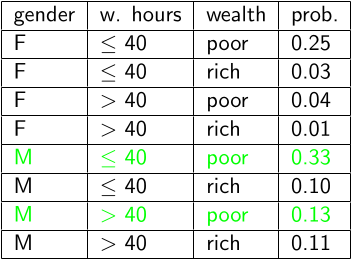
\includegraphics[width=6cm]{jd_ex.png}
        \end{center}
    

    we have: $P(M, poor) = 0.33 + 0.13 = 0.46$
}

\subsection{Inference with the Joint distribution}
Here are with the inference:
\dfn{Contintional probability}{
    Let \( E_1 \) and \( E_2 \) be two events defined as logical conditions over subsets of the random variables (e.g., \( E_1: X_i = a, X_j = b \); \( E_2: Y = y \))

    Then, \textit{conditional probability} of \( E_1 \) given \( E_2 \) is:
    \[
        P(E_1 \mid E_2) = \frac{P(E_1 \land E_2)}{P(E_2)} = 
        \frac{\displaystyle\sum_{{row} \in (E_1 \land E_2)} P({row})}
        {\displaystyle\sum_{{row} \in (E_2)} P({row})}
    \]
}

for instance:
\ex{Conditional probability}{
    Let's compute $P(M|poor ) =\frac{P(M \land poor)}{P(poor)}$. We know that $P(M, poor ) = 0.46$. Let us compute $P(poor )$:
    \begin{center}
        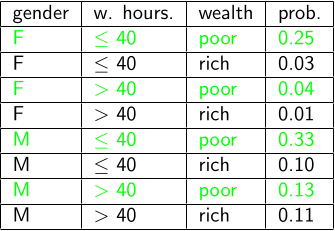
\includegraphics[width=6cm]{joint_inf.png}
    \end{center}
    Easy! $P(poor) = .75 \land P(M|poor) = 0.46/0.75 = 0.61$
}

\subsection{Complexity issues}
Let us build the joint table relative to
\[
    P(Y = wealth|X_1 = gender , X_2 = orelav.)
\]

\begin{center}
    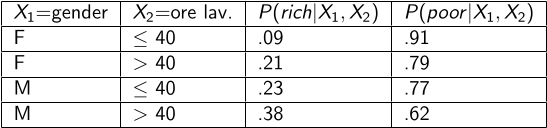
\includegraphics[width=6cm]{comp_issue.png}
\end{center}
To fill the table we need to compute $4=2^2$ parameters

If we have $n$ random variable $X = X_1 \times X_2 ,\dots, X_n$ where each $X_i$ is
boolean, we need to compute $2^n$ parameters. These parameters are \textit{probabilities}: to get reasonable value we would need a huge amount of data.

In particular the The Joint Distribution Requires \textit{Exponential parameters}
\ex{features and params}{
    \begin{itemize}
        \item With just 10 binary features, you need $2^{11}-1=2047$ parameters
        \item With 20 features: over 1 million parameters
        \item With 100 features: $2^{101}$ a number larger than the estimated atoms in the observable universe.
    \end{itemize}
}
This is computationally and statistically infeasible.
\subsubsection{USing Bayes}
for reducing complexity, we can rewrite the formula with the Bayes' rule:
\[
    P(Y=y_i\mid X=x_j) = \frac{P(Y=y_i)\cdot P(X = x_j\mid Y = y_i)}{\sum_i P(Y=y_i)\cdot P(X=x_j \mid Y=y_i)}
\]
generalising:
\[
    P(Y \mid X_1, X_2, \dots, X_n) = \frac{P(Y) \cdot P(X_1, X_2, \dots, X_n \mid Y)}{P(X_1, X_2, \dots, X_n)}
\]

But... there is a problem, it's required to know 
\[
    P(X_1, X_2, \dots, X_n \mid Y)
\]

that is the joint distribution of the features given $Y$, that requires, another time, $2^n$ params

\subsection{Naive Bayes}
For atteniung the complexity, it's possible assume an indipendencies conditional hypotesis, called "Naïve Bayes":
\[
    P(X_1,X_2,\dots,X_n|Y)=\prod_{i}P(X_i |Y)
\]
So given $Y$, $X_i$ and $X_j$ are independent from each other. In other therms:
\[
    P(X_i|X_j,Y)=P(X_i|Y)
\]
\nt{
    This means: onece we know $Y$, the feature $X_i \forall i$ are independents between each others
}
\ex{example 1}{
    A box contains two coins: a regular coin and a fake two-headed coin ($P(H) = 1$).Choose a coin at random, toss it twice and consider the following events:

    \begin{itemize}
        \item $A =$ First coin toss is H
        \item $B =$ Second coin toss is H
        \item $C =$ First coin is regular
    \end{itemize}
}
\ex{example 2}{
    For individuals, height and vocabulary are not independent, but they are if age is given.
}

\subsubsection{Giga formula with naive bayes}
\thm{Bayes rule}{
    \[
       P(Y = y_i \mid X_1, \dots, X_n) = \frac{P(Y = y_i) \cdot P(X_1, \dots, X_n \mid Y = y_i)}{P(X_1, \dots, X_n)}
    \]
}
\pf{Proof}{
    Left to mesco as exercice
}

\thm{Naïve Bayes}{
    \[
    P(Y = y_i \mid X_1, \dots, X_n) = \frac{P(Y = y_i) \cdot \prod_j P(X_j \mid Y = y_i)}{P(X_1, \dots, X_n)}
    \]
}
\pf{Proof}{
    Left to Bonzo as exercice
}

\thm{Classification of a new sample $x^{\text{new}} = \langle x_1, \dots, x_n \rangle$}{
    \label{thm:cne}
    Given a new instance represented by the feature vector $x^{\text{new}} = (x_1, x_2, \dots, x_n)$, 
    the predicted class is obtained as:
    \[
        Y^{\text{new}} = \arg\max_{y_i} \, P(Y = y_i) \cdot \prod_{j} P(X_j = x_j \mid Y = y_i)
    \]
}

\pf{Proof}{
  Seen as, using Bayes' formula, $ \forall i $ the denominator used to calculate $ P(Y = y_i | X_1, ..., X_n) $ remains the same,if we're only interested in maximizing the probability it's possible to only consider the numerator.

  Given $ P(X_1, ..., X_n) = C $, 
  \begin{align*}
    P(Y = y_i)\cdot \prod_{j}P(X_j | Y = y_i) &= C\cdot \frac{P(Y = y_i)\cdot \prod_{j}P(X_j | Y = y_i)}{C} \\
    &= C \cdot P(Y=y_i | X_1,...,X_n) \\
  \end{align*}

  Because $ C $ is a positive constant for each $ y_i $, $ arg max_{y_i} P(Y=y_i | X_1,...,X_n) = arg max_{y_i} C \cdot P(Y=y_i | X_1,...,X_n) $.
}

\nt{
    Theorem~\ref{thm:cne} expresses the decision rule of the Naïve Bayes classifier.
    Given a new vector of features $x^{\text{new}} = (x_1, x_2, \dots, x_n)$, 
    we estimate the most probable class $y_i$ by maximizing the posterior probability 
    $P(Y = y_i \mid X_1 = x_1, \dots, X_n = x_n)$, 
    which—under the conditional independence assumption—reduces to the product of the prior $P(Y = y_i)$ 
    and the individual likelihoods $P(X_j = x_j \mid Y = y_i)$.
}

\section{Learning algorithm}
Given discrete Random Variables $X_i, Y$, there are two phases
\begin{itemize}
    \item \textbf{Training}: in this phases the maching learn from the data of training set, estimating two types of probs:
    \begin{itemize}
        \item \textbf{Prior} (prob of the classes). For any possible value $y_k$ of $Y$ , estimate
        \[
            \pi_k = P(Y = y_k)
        \]
        example: if 9 out of 14 matches are "Play = Yes", then $\pi_{yes}= \frac{9}{14},\quad \pi_{no}= \frac{5}{14} $

        \item \textbf{Likelihoods}:(conditional probabilities of features). for any possible value $x_{ij}$ of $X_i$ estimate:
        \[
            \theta_{ijk} = P(X_i = x_{ij}\mid Y = y_k)
        \]
        It's the probability that a certain feature $X_i$ assumes the value $X_{ij}$, given $y_k$.

        example: $P(Outlook=Sunny\mid Play=Yes)=\frac{2}{9}$
    \end{itemize}
    \item \textbf{Classification of $a^{new} = \langle a_1 , \dots a_n \rangle$} (a vector with $n$ observed values (one for each feature)). We want to establish which class it belong to
    
    decision-making formula:
    \[
    \begin{aligned}
    Y^{\text{new}} &= \arg \max_{y_k} P(Y = y_{k}) \cdot \prod_{i} P(X_{i} = a_{i} \mid Y = y_{k}) \\
    &= \arg \max_{k} \pi_{k} \prod_{j} \theta_{ijk}
    \end{aligned}
    \]

    where:
    \begin{itemize}
        \item $P(Y=y_k)$: prior
        \item $P(X_i=a_i\mid Y=y_k)$: likelihood for each features
        \item the prod $\prod_{i}$ is given by Naive assumption
    \end{itemize}
\end{itemize}

\ex{a good day to play tennis?}{
    we wanna build a model that, given certain weather conditions, predict whether it is a good day to play tennis or not 
    
    Our class variable is:
    \[
        Y=Play\in\{Yes,No\}
    \]
    and the features observed are:
    \[
        X_1 = Outlook \quad X_2 = Temp \quad X_3=Humidity \quad X_4=Wind
    \]

    Here we have the dataset:
    \begin{table}[H]
\centering
\caption{Dataset for the \textit{Play Tennis} classification problem}
\label{tab:play_dataset}
\begin{tabular}{ccccc}
\toprule
Outlook & Temp & Humidity & Wind & Play \\
\midrule
Sunny & Hot & High & Weak & No \\
Sunny & Hot & High & Strong & No \\
Overcast & Hot & High & Weak & Yes \\
Rain & Mild & High & Weak & Yes \\
Rain & Cool & Normal & Strong & No \\
Overcast & Cool & Normal & Strong & Yes \\
Sunny & Mild & High & Weak & No \\
Sunny & Cool & Normal & Weak & Yes \\
Rain & Mild & Normal & Weak & Yes \\
Sunny & Mild & Normal & Strong & Yes \\
Overcast & Mild & High & Strong & Yes \\
Overcast & Hot & Normal & Weak & Yes \\
Rain & Mild & High & Strong & No \\
\bottomrule
\end{tabular}
\end{table}

TODO: TABELLA FATTA FARE DA UN LLM NON È VENUTA BENISSIMO

    \textbf{Calculating the prior}

    From the dataset we can compute the prior probabilities of the class variable $Y$:

    \[
    P(Y = \text{Yes}) = \frac{9}{14}, \qquad
    P(Y = \text{No}) = \frac{5}{14}.
    \]

    These represent the empirical frequencies of the two possible outcomes of $Y$.

    \medskip
    \textbf{Calculating the likelihoods}

    For each feature $X_i$ and each class $Y = y_k$, we estimate the conditional probabilities
    \[
    P(X_i = x_{ij} \mid Y = y_k),
    \]
    that is, the probability of observing a certain feature value $x_{ij}$ given that the class is $y_k$.

    For example:

    \[
    P(\text{Outlook} = \text{Sunny} \mid Y = \text{Yes}) = \frac{2}{9}, \qquad
    P(\text{Outlook} = \text{Sunny} \mid Y = \text{No}) = \frac{3}{5}.
    \]

    These values are computed as the relative frequencies in the dataset.

    \medskip
    \textbf{Classification of a new instance}

    Suppose we want to classify the new day
    \[
    x^{\text{new}} = (\text{Outlook} = \text{Sunny},\ 
    \text{Temp} = \text{Cool},\ 
    \text{Humidity} = \text{High},\ 
    \text{Wind} = \text{Strong}).
    \]

    We apply the Naïve Bayes decision rule:
    \[
    Y^{\text{new}} = 
    \arg\max_{y_i} P(Y = y_i) 
    \cdot 
    \prod_j P(X_j = x_j \mid Y = y_i).
    \]

    \medskip
    For $Y = \text{Yes}$:
    \[
    P(\text{Yes}) \cdot P(\text{Sunny}|\text{Yes}) \cdot P(\text{Cool}|\text{Yes}) 
    \cdot P(\text{High}|\text{Yes}) \cdot P(\text{Strong}|\text{Yes})
    = \frac{9}{14} \cdot \frac{2}{9} \cdot \frac{3}{9} \cdot \frac{3}{9} \cdot \frac{3}{9} 
    \approx 0.0053
    \]

    For $Y = \text{No}$:
    \[
    P(\text{No}) \cdot P(\text{Sunny}|\text{No}) \cdot P(\text{Cool}|\text{No}) 
    \cdot P(\text{High}|\text{No}) \cdot P(\text{Strong}|\text{No})
    = \frac{5}{14} \cdot \frac{3}{5} \cdot \frac{1}{5} \cdot \frac{4}{5} \cdot \frac{3}{5} 
    \approx 0.0205
    \]

    \medskip
    \textbf{Decision:}

    Since
    \[
    P(Y = \text{No} \mid x^{\text{new}}) > P(Y = \text{Yes} \mid x^{\text{new}}),
    \]
    the predicted class is
    \[
    Y^{\text{new}} = \text{No}.
    \]

    \medskip
    Therefore, according to the Naïve Bayes model, it is \textbf{not a good day to play tennis}.
}

\section{Generative techniques}
When we want to classify data (determine which category Y something belongs to given its features X), there is a fundamentally philosophical approaches, the \textbf{Generative Approach} that "learn how each class generates data", here is a sketch:
\begin{itemize}
    \item Ask: "How does each class produce its characteristic data?"
    \item Model: $P(X|Y)$ (probability of features given category)
    \item Then use Bayes' Rule to reverse it and get $P(Y|X)$
\end{itemize}

The term "Generative" come from the fact we're modeling the data generation process. We're essentially saying: "if I knew the category $Y$, I could generate/simulate typical data $X$ from that category"

\subsection{Big example: the visual intuition}
We want to calssify images into categories $\{0,1,\dots,9\}$ The generative approach says: "for each digit, learn waht imgs form that category typically look like. Then given a new img, see which category would most naturally produce such an img"

\begin{center}
    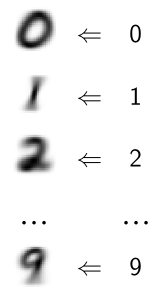
\includegraphics[width=6cm]{digit_distribution.png}
\end{center}

Okay, now we want to classify a new img:
\begin{center}
    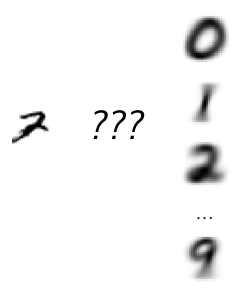
\includegraphics[width=6cm]{digit_seven.png}
\end{center}
\textbf{Which of these distributions would most likely have generated this image?}

Mathematically, for each category k:
\[
    \begin{aligned}
        \text{Score for category k} &= P(Y = k) \cdot P(X = \text{image} | Y = k)\\
                     &= \text{Prior} \cdot \text{Likelihood}
    \end{aligned}
\]

You pick the category with the highest score. You're asking which generative mode (which category's distribution) best explains the observed data

\nt{
    The "score" is just the numerator of byes rule:
    \[
        P(Y = k | X=\text{image}) = [P(Y = k) \cdot P(X=\text{image} | Y = k)] / P(X=\text{image})
    \]
}

\subsubsection{Joint Distribution vs. Naïve Bayes}
Ideally we'd want to model the Complete joint distribution:
\[
    P(X_1, X_2, \dots, X_n | Y = y_i)
\]
For MNIST, this would be the distribution of all $784$ pixels ($28\times 28$ image) for images of each digit. This distribution would capture all the correlations between pixels - how pixel 1 relates to pixel 2, how groups of pixels form edges and curves, etc. Howver, modeling the full joint distribution for $784$ dimensions is impossibly complex. We'd need:
\begin{itemize}
    \item $2^{784}$ parameters just for binary pixels (more than atoms in the universe!)
    \item An astronomical amount of training data
\end{itemize}

So we play the card "Naïve Bayes" with 2500 atk and 1000 def:
\[
    P(X_1,\dots, X_n \mid y=y_i) \approx \prod_{j} P(X_j\mid Y=y_i)
\]

The assumption (effect) is: Given the category $Y$, all pixels are \textit{independent}. This means we model each pixel separately:
\[
    \begin{aligned}
        &P(X_1 | Y = 0), P(X_2 | Y = 0), ..., P(X_{784} | Y = 0)  \\
        &P(X_1 | Y = 1), P(X_2 | Y = 1), ..., P(X_{784} | Y = 1)  
    \end{aligned}
\]
This is computationally feasible, but we've lost all information about how pixels relate to each other!
\subsection{Caution 1: The Zero Probability Problem}

From a previous example if we have $P(Play = No|Outlook = Overcast)$ the result is $\theta_Overcast,No = 0$, This happened because in our training data, we never observed a "No" (don't play tennis) when the outlook was overcast

\nt{
    Remember the classification formula:
    \[
        \text{Score} = \pi_k \cdot \prod_{i} \theta_{ijk}
    \]
    If any single $\theta_{ijk}= 0$, the entire product becomes zero. So A single feature value you've never seen in training can completely eliminate a category from consideration, even if all other features strongly support it!
}

\subsection{Caution 2: The Independence Assumption}
Naïve Bayes assumes events are independent from each other (given Y). What if this is not the case?

\subsubsection{The XOR Problem: A Fatal Limitation}

Consider random binary images where pixels are either 0 or 1. We classify based on two pixels: $p_1$ and $p_2$.

\textbf{Classification rule:}
\begin{itemize}
    \item \textbf{Category A:} if $p_1 = p_2$ (both same) — Images: $\{(0,0), (1,1)\}$
    \item \textbf{Category B:} if $p_1 \neq p_2$ (different) — Images: $\{(0,1), (1,0)\}$
\end{itemize}

This is an \textbf{XOR (exclusive OR)} relationship — a simple logical rule.

\textbf{What Naïve Bayes learns:}

For Category A (training: $(0,0)$ and $(1,1)$):
\begin{align*}
P(p_1 = 1 \mid A) &= \frac{1}{2} \quad \text{[one out of two has } p_1=1\text{]} \\
P(p_2 = 1 \mid A) &= \frac{1}{2} \quad \text{[one out of two has } p_2=1\text{]}
\end{align*}

For Category B (training: $(0,1)$ and $(1,0)$):
\begin{align*}
P(p_1 = 1 \mid B) &= \frac{1}{2} \quad \text{[one out of two has } p_1=1\text{]} \\
P(p_2 = 1 \mid B) &= \frac{1}{2} \quad \text{[one out of two has } p_2=1\text{]}
\end{align*}

\textbf{Result:} All probabilities are identical! For any test image $(a,b)$:
\begin{align*}
\text{Score}_A &= P(A) \cdot P(p_1=a \mid A) \cdot P(p_2=b \mid A) = 0.5 \cdot 0.5 \cdot 0.5 = 0.125 \\
\text{Score}_B &= P(B) \cdot P(p_1=a \mid B) \cdot P(p_2=b \mid B) = 0.5 \cdot 0.5 \cdot 0.5 = 0.125
\end{align*}

\textbf{Naïve Bayes cannot distinguish the categories!} It achieves only 50\% accuracy (random guessing) despite the trivially simple classification rule.

\textbf{Why?} The features $p_1$ and $p_2$ are \textbf{not independent} given the category — they're perfectly correlated:
\begin{itemize}
    \item In Category A: if $p_1 = 0$ then $p_2 = 0$ (with certainty)
    \item In Category B: if $p_1 = 0$ then $p_2 = 1$ (with certainty)
    \item $P(p_2 = 1 \mid p_1 = 1, A) = 1 \neq P(p_2 = 1 \mid A) = 0.5$ — violates independence!
\end{itemize}

\textbf{General lesson:} Naïve Bayes cannot learn relationships between features. It only learns how common each individual feature value is within each class, not how features combine, interact, or correlate.

\section{About Maximum Likelihood Estimation (MLE)}

\subsection{Problem definition}
In words, the Maximum Likelihood Estimation (MLE) is the parameter value that maximizes the probability of observing the given data. For instance, if we have a model where all possible outcomes are $0$ or $1$, the parameter to estimate is computed using the \textit{Bernoulli distribution}\footnote{If you don't know this, please read the \textit{Basta - Giolapalma notes for probability}} $P(w) = \theta^w (1-\theta)^{(1-w)}$ where $w\in\{0,1\}$ represents all possible outcomes. However, normally we have a dataset (in this case a sequence of observations $D = \{w_1, w_2, \ldots, w_n\}$) and we don't know $\theta$. The goal is to find the value of $\theta$ that makes our observed sequence most probable.

For independent observations, the likelihood is:
\[
    L(\theta|D) = P(D|\theta) = \prod_{i=1}^n P(w_i|\theta) = \prod_{i=1}^n \theta^{w_i}(1-\theta)^{1-w_i}
\]

Let $\alpha_0 = \sum_{i=1}^n w_i$ be the number of times we observed $1$ (successes), and $\alpha_1 = n - \alpha_0$ be the number of times we observed $0$ (failures). Then:
\[
    L(\theta|D) = \theta^{\alpha_0}(1-\theta)^{\alpha_1}
\]

The MLE is obtained by maximizing this likelihood (or equivalently its logarithm) with respect to $\theta$.

\dfn{MLE}{
    Given:
    \begin{itemize}
        \item A parametric probability model with parameter(s) $\theta$
        \item Observed data $D=\{x_1, \dots, x_n\}$
        \item A likelihood function $L(\theta|D) = P(D|\theta)$ (probability of data given parameters)
    \end{itemize}

    The \textit{Maximum Likelihood Estimator} is defined as:
    \begin{center}
        \begin{math}
           \hat{\theta}_{MLE} = \arg\max_\theta{L(\theta\mid D)} = \arg \max_\theta P(D|\theta)
        \end{math}
    \end{center}

    In words: $\hat{\theta}_{MLE}$ is the parameter value that maximizes the probability of observing the given data.
}

\subsection{Results for Bernoulli}



\thm{MLE for Bernoulli}{
    Given a set of $n$ i.i.d. (independent and identically distributed) observations $D = \{w_1, \ldots, w_n\}$ from a Bernoulli distribution with parameter $\theta$. The Maximum Likelihood Estimate (MLE) for $\theta$ is the sample frequency of successes.
    
    If $\alpha_0$ is the number of successes (observations equal to 1), then the estimate is given by:
    \[
        \hat{\theta}_{MLE} = \frac{\alpha_0}{n}
    \]
}


\pf{Derivation for Bernoulli}{
    For independent Bernoulli trials with outcomes $w_i \in \{0,1\}$, the likelihood is:
    \[
        L(\theta|D) = \prod_{i=1}^n P(w_i|\theta) = \prod_{i=1}^n \theta^{w_i}(1-\theta)^{1-w_i}
    \]
    
    Let $\alpha_0 = \sum_{i=1}^n w_i$ (number of $1$'s) and $\alpha_1 = n - \alpha_0$ (number of $0$'s). Then:
    \[
        L(\theta|D) = \theta^{\alpha_0}(1-\theta)^{\alpha_1}
    \]
    
    Taking the logarithm (which preserves the maximum since $\log$ is monotonically increasing):
    \[
        \ell(\theta) = \log L(\theta|D) = \alpha_0 \log(\theta) + \alpha_1 \log(1-\theta)
    \]
    
    To find the maximum, take the derivative and set to zero:
    \[
        \frac{d\ell}{d\theta} = \frac{\alpha_0}{\theta} - \frac{\alpha_1}{1-\theta} = 0
    \]
    
    Solving:
    \begin{align*}
        \frac{\alpha_0}{\theta} &= \frac{\alpha_1}{1-\theta} \\
        \alpha_0(1-\theta) &= \alpha_1\theta \\
        \alpha_0 &= \theta(\alpha_0 + \alpha_1) \\
        \hat{\theta}_{MLE} &= \frac{\alpha_0}{\alpha_0 + \alpha_1} = \frac{\alpha_0}{n}
    \end{align*}
    
    To verify this is a maximum, check the second derivative:
    \[
        \frac{d^2\ell}{d\theta^2} = -\frac{\alpha_0}{\theta^2} - \frac{\alpha_1}{(1-\theta)^2} < 0
    \]
    Since the second derivative is negative for $\theta \in (0,1)$, this confirms a maximum
}

\subsection{Multivalued case}
Now I presented the formula just for two possible cases using the Bernoulli distribution, and for multivalued cases? WE HAVE THE \textit{multinomial distribution}

\nt{Multinomial distribution is $P(X^n = \alpha_i\mid \theta) = c_{\alpha_i} \prod_{i}\theta_{i}^{\alpha_i}$. where $\alpha_i$ is the number of i in the sequence and $ c_{a_i}$ is a combinatorial constant not depending on $\theta$
}

\thm{MLE for Discrete Distributions}{
    The Maximum Likelihood Estimate (MLE) for the probability $\theta_i$ of each outcome is its observed sample frequency.

    If $\alpha_i$ is the number of times the i-th outcome has been observed in the $n$ trials, then the estimate for its probability is:
    \[
        \hat{\theta}_i = \frac{\alpha_i}{n}
    \]
}
\pf{Proof}{
    Basta exercice
}

\cor{MLE for Naïve Bayes Parameters}{
    As a direct consequence of the main theorem, the Maximum Likelihood Estimates for the parameters of a Naïve Bayes classifier are also given by their sample frequencies:

    \begin{enumerate}
        \item ($\pi_k$) The MLE for the prior probability of a class $y_k$ is its relative frequency in the dataset. 
        \[
            \hat{\pi}_k = P(Y = y_k) = \frac{\#\mathcal{D}\{Y = y_k\}}{|\mathcal{D}|}
        \]

        \item ($\theta_{ijk}$) The MLE for the conditional probability of a feature $X_i$ taking the value $x_{ij}$ given a class $y_k$, is the relative frequency of that feature value within the subset of data belonging to class $y_k$.
        \[
            \hat{\theta}_{ijk} = P(X_i = x_{ij} | Y = y_k) = \frac{\#\mathcal{D}\{X_i = x_{ij} \land Y = y_k\}}{\#\mathcal{D}\{Y = y_k\}}
        \]
    \end{enumerate}
}
\section{Document classification with Bag of Words (BoW) approach}
The Bag-of-Words ($BoW$) model is a technique for document classification, which involves assigning a document to a predefined category (like Sport, politics, Tech, ect...). The core idea is to treat a doc not like a sorted sequence of phrases but like a simple Bag where words have no order or grammar, in this technique the primary focus is on capturing the occurrence frequency of each word within the document (this is a very surface level method that doesn't consider things like sarcasm and negation).

So we assume that:
\begin{itemize}
  \item words are the elementary value of events ($ X_i $ is the i-th word in the document): $ \theta_{i, j, k} = P(X_i = x_j | Y = y_k) $, where $ x_j $ is the $ j $-th distinct word contained somewhere in the document and $ y_k $ is the $ k $-th category\footnote{Words and categories aren't ordered in any particular way.}.
\item events are independent (given the category
  \footnote{Obviously, knowing a word in the document will give information regarding the type of the document (this is the notion that the model relies on), thus changing the distribution for all the other positions. For this reason we say that events are independent \textit{only} if the category is considered known.}
  ): $ \forall i,j,m,n,k. i \neq m.\  P(X_i = x_j | X_m = x_n, Y = y_k) = \theta_{i,j,k} $
  \item distribution is independent from the position: $ \forall i,m,j,k. \ \theta_{ijk} = \theta_{mjk} $
\end{itemize}


\subsection{Training and classification}
Event $X_i=$ i-th word in the document: a discrete random variable assuming as many values as words in the language
\[
    \theta_{i,j,k} = P(X_i = x_j \mid Y = y_k)
\]
In words: "the probability that in a document of the category $y_k$ the word
$ x_j $ appears at position $i$", but for the BoW technique we assume that we have a distribution independent from the position and that all event are independents so 
\[
  \theta_{i,j,k} =  \theta_{m,j,k}= \theta_{j,k}
\]
For this reason, we can just consider the stochastic variable $ X = \text{"word randomly extracted from document"} $, with $ \theta_{j, k} = P(X = x_j | Y = y_k) $.
Then with discrete random variables $X$, $Y$ let's define the training and classification:
\begin{itemize}
    \item \textbf{Training}: 
    \begin{itemize}
      \item for any possible value $y_k$ of $Y$, estimate the prior
        \[
            \pi_k=P(Y=y_k)
        \]
      \item for each distinct word in the document $ x_j $, estimate the likelyhood:
        \[
            \theta_{jk} = P(X = x_j \mid Y = y_k )
        \]
        (the condition prob that a certain word $x_j$ appears in a doc, knowing that that doc belongs to category $y_k$)
    \end{itemize}
    \item \textbf{Classification of} $a^{\texttt{new}} = \langle a_1,\dots,a_n \rangle$ (new sequence of words):
    \begin{align*}
        Y^{\texttt{new}} &=\arg\max_{y_k} P(Y = y_k) \cdot \prod_{i=1}^n P(X = a_i | Y = y_k)\\
        &= \arg\max_{k}\pi_k\cdot \prod_{i=1}^{n}\theta_{j(i),k}
    \end{align*}
    where $j(i)$ is such that $ x_{j(i)} = a_i $.
\end{itemize} 

The probabilities needed for the classifier are estimated from the dataset using Maximum Likelihood Estimates (MLE's):
\begin{itemize}
    \item The MLE for the prior probability of a class, $\pi_k$, is the fraction of the documents in the training set that belong to category $y_k$
    \item The MLE for the conditional probability of a word, $\theta_{\text{\texttt{word}},k}$, is the frequency of that word within all documents belonging to category $y_k$
\end{itemize}
The classification formula involves multiplying many small probabilities, which can lead to numerical instability (underflow). To solve this, we can maximize the logarithm of the likelihood instead, since the logarithm is a monotonically increasing function and will not change the location of the maximum.

The classification rule becomes:
\[
  Y^{\texttt{new}} = \arg\max_{y_k} \left( \log(\pi_k) + \sum_i \log(\theta_{j(i)k}) \right)
\]
This can be further simplified by grouping identical words (values of $ i $ with the same $ j(i) $). If $n_j$ is the number of occurrences of the unique word $x_j$ in the new document, the sum becomes a weighted sum:
\[
  \sum_i \log(\theta_{j(i)k}) = \sum_j n_j \cdot \log(\theta_{jk})
\]
This final expression can be elegantly interpreted as a dot product in a high-dimensional vector space where each word of the vocabulary is a dimension

\subsection{Dot product, correlation, Cosine similarity}
the core idea is manipulating texts in numerical vectors. For doing this, you can create a vectorial space at $n-$dimension where each dimension correspond to a word to one unique word of vocabulary. HEre is the training and classification:
\begin{itemize}
    \item \textbf{Training}
    For any category $k$ build a “spectral” vector
    \begin{center}
        \begin{align*}
            s_k =\langle  \log_{(\theta_{jk})} \rangle
        \end{align*}
    \end{center}

    $\theta_{jk}=$ frequency of the word j in documents of the category k

    For each category (ex. "Sport") we'll create a spectral vector where each componet of this vector is the log of the probs ($\log{(\theta_{jk})}$) of a specific category. This vector represent the "profile" or carateristic direction of that category in the space of words

    
    \item \textbf{classification}
    Given a new doc, compute a vector
    \[
        d = \langle n_j \rangle_{j\in \texttt{words}}
    \]
    and classify the doc as
    \[
        \arg \max_k d\cdot s_k =\sum_{j}d_j\cdot s_{jk}
    \]
    so we're searching for the value of $ k $ that leads to the highest \textit{correlation} between the two vectors.
\end{itemize}

\subsubsection{geometrically and analytically}
\dfn{Dot product - Geometric def}{
    We define \text{dot product} 
    \begin{center}
        \begin{math}
            \textbf{a}\cdot \textbf{b} = |\textbf{a}|\cdot| \textbf{b}|\cos(\theta)
        \end{math}
    \end{center}
}

\dfn{Dot product - Analytic definition}{
    given $\vectdef{a}, \vectdef{b}$
    \[
           \textbf{a}\cdot\textbf{b} = \sum_{i=1}^{n}a_ib_i
    \]
}


The dot product can be influenced by the length of docs (a longer doc can have high frequencies). The cosine similarity resolve this problem normalizing the dot procd respect to the lenght of two vectors
\[
    S_c (\textbf{a}, \textbf{b}) = \cos(\theta) = \frac{\textbf{a}\cdot\textbf{b}}{\|\textbf{a}\|\cdot\|\textbf{b}\|}
\]

the results is a value $\in[-1,1]$ that measures the "similarity of direction" ignoring the length. A value of 1 means that the vectors points in the same direction

\ex{Vector correlation maximization}{
 \begin{center}
   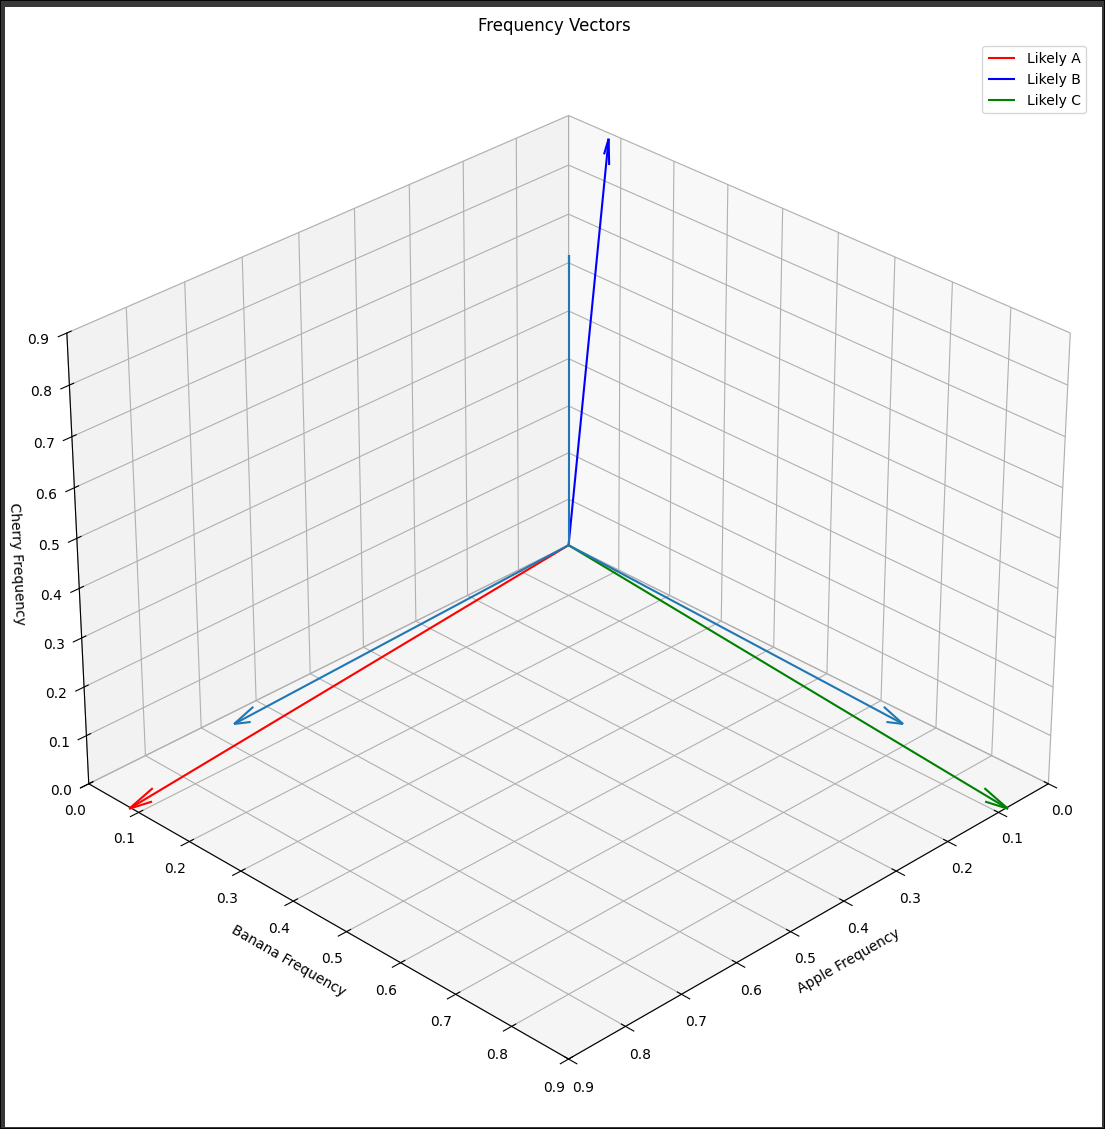
\includegraphics[width=0.5\textwidth]{img/2025-10-19-17-23-00.png}
 \end{center} 

 This is an example in 3 dimensions showing how the BoW approach can be seen as minimizing the angle between vectors (or maximizing their correlation)
}

\thm{Equivalence of Dot Product Definitions}{
    The geometric definition of the dot product, $\vec{a} \cdot \vec{b} = |\vec{a}||\vec{b}|\cos(\theta)$, is equivalent to the analytic definition, $\vec{a} \cdot \vec{b} = \sum_{i=1}^n a_i b_i$.
}
\pf{Proof}{


The proof begins with the \textit{Carnot's theorem}, which generalizes the Pythagorean theorem. Consider the triangle formed by the vectors $\vec{a}$, $\vec{b}$, and their difference, $\vec{a} - \vec{b}$.

The Law of Cosines states:
\[
|\vec{a} - \vec{b}|^2 = |\vec{a}|^2 + |\vec{b}|^2 - 2|\vec{a}||\vec{b}|\cos(\theta)
\]
Here, the term $|\vec{a}||\vec{b}|\cos(\theta)$ corresponds to the geometric definition of the dot product, $\vec{a} \cdot \vec{b}$. By rearranging the formula algebraically, we can express the dot product in terms of vector magnitudes:
\[
\vec{a} \cdot \vec{b} = \frac{|\vec{a}|^2 + |\vec{b}|^2 - |\vec{a} - \vec{b}|^2}{2}
\]

Next, we substitute the analytic definition of the squared magnitude of a vector. For simplicity, let's consider the two-dimensional case where $\vec{a} = [a_1, a_2]$ and $\vec{b} = [b_1, b_2]$. We have:
\begin{align*}
|\vec{a}|^2 &= a_1^2 + a_2^2, \\
|\vec{b}|^2 &= b_1^2 + b_2^2, \\
|\vec{a} - \vec{b}|^2 &= (a_1 - b_1)^2 + (a_2 - b_2)^2.
\end{align*}

Substituting these into the dot product expression yields:
\[
\vec{a} \cdot \vec{b} = \frac{(a_1^2 + a_2^2) + (b_1^2 + b_2^2) - \left( (a_1 - b_1)^2 + (a_2 - b_2)^2 \right)}{2}.
\]

Expanding the squared terms in the numerator:
\[
\vec{a} \cdot \vec{b} = \frac{a_1^2 + a_2^2 + b_1^2 + b_2^2 - (a_1^2 - 2a_1b_1 + b_1^2 + a_2^2 - 2a_2b_2 + b_2^2)}{2}.
\]

Simplifying by canceling out the squared terms:
\[
\vec{a} \cdot \vec{b} = \frac{2a_1b_1 + 2a_2b_2}{2}.
\]

This simplifies to the final result:
\[
\vec{a} \cdot \vec{b} = a_1b_1 + a_2b_2.
\]

This is the analytic definition of the dot product for the two-dimensional case. The proof can be generalized to $n$ dimensions, demonstrating the equivalence of the geometric and analytic definitions of the dot product.

}

\section{The linear nature of Naive Bayes (boolean case)}

If both $ X_i $ and $ Y $ are boolean variables, it's possible to transform the Naive Bayes formula using certain properties of boolean functions to obtain a \textit{linear} expression.

\thm{Linarity of classifier Naive bayes for boolean feature}{

}

Given $X_i, Y$ booleans, the classification of a new $\vec{x} = \langle x_1,\dots, x_n\rangle$ happens comparing the probs that $x$ belong to class $1$ and $0$:
\[
    \frac{P(Y=1 \mid X_1 \dots X_n = \vec{x})}{P(Y=0 \mid X_1 \dots X_n = \vec{x})} = \frac{P(Y=1)\prod_{i}P(X_i = x_i\mid Y=1)}{P(Y=10\prod_{i}P(X_i = x_i\mid Y=0} \geq 1
\] 
if the results is $\geq 1$ we choose the class one.

Passing to logarithms we have:
\[
    \log{\frac{P(Y=1)}{P(Y=0)} + \sum_i\frac{X_i=x_i\mid Y=1}{X_i=x_i\mid Y=0}}\geq 0
\]
if the results is $\geq 0$ we choose the class one. 

Now define the conditional probs loke $\theta_{ik} = P(X_i = 1\mid  Y=k)$. Of consequence, $P(X_i = 0 \mid Y=k)=1-\theta_{ik}$. The generic therm of the sum, $\log{\frac{P(X_i =x_i\mid Y=1)}{P(X_i =x_i\mid Y=0)}}$, using the fact that for a boolean function $f(x)=xf(1)+(1-x)f(0)$ we have:
$$
    \sum_i \left( x_i \cdot \log\frac{P(X_i=1|Y=1)}{P(X_i=1|Y=0)} + (1-x_i) \cdot \log\frac{P(X_i=0|Y=1)}{P(X_i=0|Y=0)} \right)
$$
    with $\theta$, the expression becomes:
$$
    \log\frac{P(Y=1)}{P(Y=0)} + \sum_i \left( x_i \cdot \log\frac{\theta_{i1}}{\theta_{i0}} + (1-x_i) \cdot \log\frac{1-\theta_{i1}}{1-\theta_{i0}} \right) \ge 0
$$
that is a linear expression in the set of features $x_i$ in the form
\[
    w_0 + \sum_i w_i x_i \geq 0
\]
Classification algorithms based on a linear combination of the
features values.
Every feature is evaluated independently from the others and
contributes to the result in a linear way, with a suitable weight
(that is a parameter of the model, to be estimated).
For instance, if the features are pixels of some image, we may use
linear methods only up some normalization (in position and
dimension) of the object to be recognized

\section{Gaussian Naive Bayes}
The standard Naïve Bayes algorithm is designed for discrete features. However, in many real-world scenarios, features can be continuous, such as the height of an individual, the temperature, or the color intensity of a pixel. For continuous variables, the probability of observing a specific value is infinitesimally small, making the pointwise probability $P(X_i | Y)$ effectively null.

To address this challenge, Gaussian Naïve Bayes extends the classifier by making a crucial assumption: that the data for each continuous feature, conditioned on a specific class, follows a \textbf{Gaussian (or Normal) distribution}
\footnote{
 The reason we make this assumption is because, given a mean and a variance, the Gaussian is the distribution with the highest entropy. This means that it makes the weakest assumptions, distributing the probability in the most even way possible for all possible results.
}. 
Instead of estimating a probability for each value, we estimate the parameters of this distribution (the mean and variance) from the training data.

\dfn{Gaussian Distribution}{
    The \textit{Gaussian Distribution} is a continuous probability distribution characterized by its mean $\mu$ and variance $\sigma^2$. Its probability density function (PDF) is given by:
    \[
        p(x | \mu, \sigma) = \frac{1}{\sigma\sqrt{2\pi}} e^{-\frac{(x-\mu)^2}{2\sigma^2}}
    \]
    where:
    \begin{itemize}
        \item The mean $E[X] = \mu$ defines the center of the distribution.
        \item The variance $\text{Var}[X] = \sigma^2$ defines the spread of the distribution.
    \end{itemize}
}

\subsection{Accuracy, Precision and Recall}
\dfn{Accuracy}{
    \[
        \texttt{Accuracy} = \frac{TP+TN}{ALL}
    \]
    number of correctly classified samples
}
\dfn{Precision}{
    \[
        \texttt{Precision} = \frac{TP}{TP+FP}
    \]
    percentage of true prositives over predicted ones
}
\dfn{Recall}{
    \[
        \texttt{Recall} = \frac{TP}{TP+FN}
    \]
    percentage of true positives over all positives
}
\dfn{}{
    \[
        F1 = 2\frac{Precision \cdot Recall}{Precision + Recall}
    \]
    harmonic mean of precision and recall
}
\subsection{Descriptive parameters of the model}
We assume (inductive bias) that for every value $y_k$ of $Y$ the
random variable $P(X_i |Y = y_k )$ has a Gaussian distribution
\[
    \mathcal{N}(x\mid \mu_{ik} \sigma-{ik}) = \frac{1}{\sigma_{ik}\sqrt{2\pi}}e^{-\frac{(x-u_{ik})^2}{2\sigma^2_{ik}}}
\]
\begin{itemize}
    \item \textbf{Learning}: estimate the values of the parameters $ \mu i k $, $\sigma_{i_k}$ and $\pi_k = P(Y = y_k )$
    \item \textbf{Classification} of $x^{new} = \langle a_1,\dots, a_n\rangle$
        \begin{align*}
            Y^{\texttt{new}} &= \arg \max_{y_k} P(Y= y_k ) \cdot \prod_{i} P(X_i = a_i \mid Y = y_k )\\
            &= \arg \max_{k}\pi_k\cdot \prod_{i}\mathcal{N}(a_i\mid \mu_{ik},\sigma_{ik})
        \end{align*}
\end{itemize}

\subsection{MLE for Gaussian Parameters}
Given a set of training data, the Maximum Likelihood Estimates (MLE) for the parameters of the Gaussian distribution for each feature $X_i$ and class $y_k$ are the sample mean and sample variance, calculated from the subset of data belonging to class $y_k$.
    
    \begin{itemize}
        \item \textbf{Mean Estimate ($\mu_{ik}$):} The mean value of $X_i$ for samples with label $Y=y_k$. Formally:
        \[
            \mu_{ik} = \frac{\sum_j X_i^j \delta(Y^j = y_k)}{\sum_j \delta(Y^j = y_k)}
        \]
        \item \textbf{Variance Estimate ($\sigma_{ik}^2$):} The variance of $X_i$ for samples with label $Y=y_k$. Formally:
        \[
            \sigma^2_{ik} = \frac{\sum_j (X_i^j - \mu_{ik})^2 \delta(Y^j = y_k)}{\sum_j \delta(Y^j = y_k)}
        \]
    \end{itemize}
    where $j$ ranges over all samples in the training set, and $\delta(Y^j = y_k)$ is the indicator function:
    \[
        \delta(Y^j = y_k) = \begin{cases} 
            1 & \text{if } Y^j = y_k \\ 
            0 & \text{otherwise} 
        \end{cases}
    \]

\section{Logistic Regression}
Logistic regression is a discriminative machine learning method used primarily for classification problems

\subsection{Core idea}
\begin{itemize}
    \item Naive Bayes allows us to compute $P(Y |X )$ after having learned $P(Y)$ and $P(X |Y)$
    \item Why not directly learn $P(Y |X )$?
\end{itemize}

\thm{The shape of $P(Y\mid X)$}{
    hypotesis:
    \begin{itemize}
        \item $Y$ boolean random variable
        \item $X_i$ continuous random variable
        \item $X_i$ independent from each other $Y$
        \item $P(X_i \mid Y = k)$ have Gaussian distributions $N(\mu_{i_k} ,\sigma_i)$(Warning not $\sigma_ik$ !)
        \item $Y$ has a Bernoulli distribution $(\pi)$
    \end{itemize}
    then
    \begin{equation}
        P(Y=1\mid X =\langle x_1 \dots x_n\rangle) =\frac{1}{1+\exp{(w_0+\sum_iw_ix_i)}}
    \end{equation}
}
\pf{Proof}{
    By hypothesis, the conditional probability of a feature $X_i$ is given by a Gaussian PDF:
    \[
        P(X_i | Y=k) = \mathcal{N}(x_i; \mu_{ik}, \sigma_i) = \frac{1}{\sigma_i\sqrt{2\pi}}e^{-\frac{(x_i-\mu_{ik})^2}{2\sigma_i^2}}
    \]
    We want to find the shape of $P(Y=1|\vec{x})$. Using the definition of conditional probability and the law of total probability, we have:
    \begin{align*}
        P(Y=1|\vec{x}) &= \frac{P(Y=1)P(\vec{x}|Y=1)}{P(\vec{x})} \\
        &= \frac{P(Y=1)P(\vec{x}|Y=1)}{P(Y=1)P(\vec{x}|Y=1) + P(Y=0)P(\vec{x}|Y=0)}
    \end{align*}
    Dividing the numerator and denominator by $P(Y=1)P(\vec{x}|Y=1)$ gives:
    \begin{align*}
        P(Y=1|\vec{x}) &= \frac{1}{1 + \frac{P(Y=0)P(\vec{x}|Y=0)}{P(Y=1)P(\vec{x}|Y=1)}} \\
        &= \frac{1}{1 + \exp\left(\ln\left(\frac{P(Y=0)P(\vec{x}|Y=0)}{P(Y=1)P(\vec{x}|Y=1)}\right)\right)}
    \end{align*}
    Using the Naïve Bayes assumption of conditional independence $P(\vec{x}|Y) = \prod_i P(x_i|Y)$ and substituting $P(Y=1)=\pi$, we get:
    \[
        P(Y=1|\vec{x}) = \frac{1}{1 + \exp\left(\ln\frac{1-\pi}{\pi} + \sum_i \ln\frac{P(x_i|Y=0)}{P(x_i|Y=1)}\right)}
    \]
    Substituting the Gaussian PDF and simplifying the term inside the summation leads to a linear function of $x_i$:
    \[
        P(Y=1|\vec{x}) = \frac{1}{1 + \exp\left(\ln\frac{1-\pi}{\pi} + \sum_i \left(\frac{\mu_{i0}-\mu_{i1}}{\sigma_i^2}x_i + \frac{\mu_{i1}^2 - \mu_{i0}^2}{2\sigma_i^2}\right)\right)}
    \]
    This expression has the form $\frac{1}{1 + \exp(z)}$, where $z$ is a linear combination of the features $x_i$. By defining $w_0$ and $w_i$ as the appropriate combinations of the Gaussian parameters ($\mu, \sigma, \pi$), we obtain the logistic form:
    \[
        P(Y=1|\vec{x}) = \frac{1}{1 + \exp(w_0 + \sum_i w_i x_i)}
    \]
}
\subsection{Training for logistic regression}
So, logistic regression assumes
\[
 P(Y=1\mid X =\langle x_1 \dots x_n\rangle) =\frac{1}{1+\exp{(w_0+\sum_iw_ix_i)}}
\]
and directly tries to estimate the parameters $w_i$ (the change in sign
is ininfluent).

\dfn{Logistic function}{
    It's a very important funcition and it's called logistic function:
    \[
        \sigma(x) = \frac{1}{1+e^{-x}}
    \]
}

With this def we know that $P(Y=1\mid x, w) = \sigma (w_0 + \sum_{i}x_iw_i)$

\subsubsection{Training via Maximum Likelihood Estimation}

Given independent training samples $\langle x^\ell, y^\ell \rangle$, we want to find the parameters $w$ that \textbf{maximize} the probability of observing our training data.

The probability of all samples is:
\[
\prod_\ell P(y^\ell | x^\ell, w) = \prod_\ell P(y^\ell = 1|x^\ell, w)^{y^\ell} \cdot P(y^\ell = 0|x^\ell, w)^{(1-y^\ell)}
\]

\nt{This formula works because when $y^\ell = 1$, only the first term contributes (the second becomes 1), and vice versa when $y^\ell = 0$.

Since $P(Y=0|x,w) = 1 - P(Y=1|x,w)$, we can write:
\[
\prod_\ell P(y^\ell | x^\ell, w) = \prod_\ell \sigma(w_0 + \sum_i w_i x_i^\ell)^{y^\ell} \cdot (1-\sigma(w_0 + \sum_i w_i x_i^\ell))^{(1-y^\ell)}
\]}

\subsubsection{Log-Likelihood}

Instead of maximizing the product directly, we \textbf{maximize the logarithm} of this probability (which is equivalent since log is monotonic):
\[
\ell(w) = \sum_\ell \log P(y^\ell | x^\ell, w) = \sum_\ell \left( y^\ell \cdot \log P(Y=1|x^\ell, w) + (1-y^\ell) \cdot \log P(Y=0|x^\ell, w) \right)
\]

\subsubsection{Gradient}

Unfortunately, there is no analytic solution for the previous
optimization problem.
so, we use iterative optimization methods, like the gradient
technique:

GRADIENTE IN CADUTA LIBERA

% \end{document}
